\documentclass[12pt]{article}

\author{Aria Koehler\\{\small Advisor: Matthew Plumlee}}
\title{Estimating Dynamical Systems Parameters with Autodifferentiation Methods}
\date{03/19/2022}

\usepackage{amsmath}
\usepackage{amssymb}
\usepackage{graphicx}
\usepackage{float}
\usepackage{hyperref}

%% \usepackage{fullpage}


\newcommand{\cn}{$^{\textit{[citation needed]}}$}
%% \usepackage{}


\begin{document}

\maketitle



%% \begin{abstract}
  
%% \end{abstract}


\section{Notation}

\begin{itemize}

\item
  $d$: Number of dimensions of state vector

\item
  $N$: Number of time points

\item
  $p$: Number of basis functions we search over when looking for unmodelled terms.

\item
  $t_i$: Time at point $i$
  
\item
  $x_i^* \in \mathbb{R}^d,\, i=1,\ldots, N$: State vector of the ``true'' model at time $t_i$. 

\item
  $x_i(\eta) \in \mathbb{R}^d,\, i=1,\ldots, N$: State vector of the approximate model at time $t_i$. 
  
\item
  $f_0: \mathbb{R}^d \to \mathbb{R}^d$: Basic model, which is known in principle.

\item
  $m^*(x, \eta): \mathbb{R}^d \to \mathbb{R}^d$: Unmodelled terms in a system, which we will call \textit{supplemental terms}. In principle not known.

\item
  $m_i(x)$: Basis functions for approximating $m^*$. Write $m(x) = \sum_{i=1}^{p} \eta_i m_i(x)$.

\item
  $f^*(x) = f_0(x) + m^*(x)$: True full model, including supplemental terms.

\item
  $f(x, \eta) = f_0(x) + m(x, \eta)$: Predicted model, including known terms and estimated supplemental  
  
\item
  $\eta \in \mathbb{R}^{p \times d}$: Parameters associated with the functions in our search basis.

\end{itemize}



\section{Introduction}

\subsection{Direction}

Dynamical systems models have been used to great effect in a variety of different fields. Though analysis of these models is well-worn, some issues remain when it comes to aligning the model to real-world data.

One is the issue of parameter estimation. Though frameworks exist for estimating the parameters of a differential equation, the problem of minimizing 2-norm between a model's predictions and a given dataset is, in general, ill-posed\cite{chung}. Thus, the problem of finding a model that minimizes the 2-norm still has challenges, even moreso for the problem of finding a model that is interpretable.

The problem is to find $f$ such that the solution $x(\eta)$ of $\dot{x} = f(x,\eta)$ approximates the solution $x^*$ of $\dot{x}* = f^*(x)$ optimally under a given loss $L(x^*, x(\eta))$ (further details on the loss later). There are a few main contributors to the model's overall loss. The sources of focus going forward are discretization error, model error, and ``true'' stochastic noise. In this paper, the issue of model error will be addressed. Model error is defined broadly to be the error in the predicted outcomes of a dynamical system due to misspecifying or underspecifying the dynamics governing the change in the state vector. For example, if one sets $\dot{x} = k x$, but in reality $\dot{x} = k x^2$, there is little hope to recover the ``true'' model by simply finding $k$.

That is, consider a vector-valued function $x$, which evolves according to $$\dot{x}(t) = f(x, \eta^*) \equiv f_0(x) + m^*(x),$$ defined on a discretized time grid $t_1, \ldots, t_N$ and a given dynamical systems model $f_0(x),$ for which there is some \textit{a priori} reason to believe is a good model for the time-evolution of $x$. Then the problem is to find $$f(x, \eta) = f_0(x) + m(x, \eta),$$ such that $L(x^*, x(\eta))$ is minimized.

One advantage of this approach in the context of a general problem is the ability to make use of both domain knowledge\---through incorporation of the initial model $f_0$\---and data by way of learning $m^*(x)$\cite{levine}.


%% The problem we will focus on primarily is the issue of determining the sources of error in dynamical systems. If a proposed model gives us a certain quantity of error, how do we know what causes that error? Is it the result of unmodelled effects in the right-hand sides of our equations? If so, can we learn those effects given a search basis $\{ m_i\}_{i=1}^p$? How much error is coming from discretizing the time steps, and can we estimate that and try to account for it when making predictions? And last, how much of the error we see can we attribute to ``true'' noise or measurement error? Many attempts have been made, with more or less success, to address these issues, but few have attempted to look at these problems in a unified way and attempted to tackle the problem of uncertainty in dynamical systems as a single problem.


These are far-reaching issues, and we will not try to solve them all in this article, but we think that approaching them as a unified problem will provide useful ways of thinking as the field progresses.


%% The dynamical systems we will look at concern the general system $$\dot{x}(t,\eta) = f(x;\eta).$$

%% Though most of these methods work in the general case, all of the systems we actually look at will have no direct dependence on $t$, so we will ignore it going forward and just write $f(x;\beta)$.


\section{Background}

\subsection{Parameter Estimation}

The first problem to be considered is that of estimating parameters $\eta^*$. That is, given $f(x,\eta)$ and a set of data $x^*_1, \ldots , x^*_N$, can an estimate of $\eta^*$ be obtained?

One such approach to this problem involves Bayesian statistical models, as in Gelman, et al. (1996). This approach begins with a prior distribution describing model parameters. The differential equations are then solved numerically under the given parameter values, and the prior distributions are updated according to a Bayesian update procedure. This approach has several advantages, in particular that it is able to account for hierarchical effects. In the particular problem considered, there are both population effects and individual effects, which can be considered at the same time with their hierarchical structure intact.\cite{gelman} However, this method also requires performing MCMC, which does not always converge in easily predictable ways, and its convergence can rarely be verified.\cite{vehtari} Primarily for this reason, we will favor methods that do not involve performing MCMC.

%% Gelman, et al. (1996) addressed a particular instance of this problem in pharmacokinetics, using a hierarchical Bayesian approach. They began with a Bayesian prior describing the parameters of their model, under which they numerically solved the dynamical systems and then used the resulting error distributions to update their paramter distributions using MCMC methods. One advantage this gave them in their particular case was that it allowed them to jointly construct a population model and individual models by exploiting the hierarchical nature of Bayesian models.\cite{gelman} However, for a general problems their method has a litany of problems, including that there are not always obvious choices of prior, and the computation of posterior is not always tractable.

More recently, more methods have arisen which rely on basis function expansions. Ramsay, et al. (2007), use one such method which treats the problem as a nested optimization. In an outer problem, updates are performed on the model parameters, optimizing the Euclidean distance between the model's predictions and observed data. The inner problem finds the coefficients for the basis functions which solve the differential equations for the current parameters.\cite{ramsay}

Even more recently, Levine and Stuart (2021) use techniques from machine learning to predict unobserved states that may affect the observed state vector. The methods are remarkably powerful and show additionally that starting with an educated guess of the true model can cause RNN predictions to reach optimality much faster than when they are given only data.\cite{levine} However, there are several questions that the authors do not answer. For example, it is not clear that these parameters are uniquely interpretable. The method might have terms that cancel each other, and the given model may be absorbed in the estimated part.

%% For example, how much uncertainty can we expect in these estimations in general? And how can we ensure that the parameters we discover, as well as our starting model, are uniquely meaningful, and that we do not just absorb the ``known'' model in our discovered model?


\subsection{Uncertainty Quantification in Numerical Solutions of ODEs}

While estimating the parameters of the ODEs themselves is a large part of this problem, it may also be useful to know how precise those estimates are. For example, Chkrebtii, et al. (2016) use a Bayesian method that conditions on model uncertainty in order to solve the system itself. They also use a quantification of model information to prove convergence properties of their algorithm, which could be challenging to show for other methods.\cite{chkrebtii} However, the use of Bayesian methods can lead to a variety of practical problems which the proposed methods will try to avoid, as noted above.

These problems are difficult to avoid, however, when quantifying uncertainty. Most current methods of uncertainty analysis require the use of Bayesian methods, largely because the posterior distribution of an estimated parameter typically comes packaged with a measure of variance. For example, Cockayne, et al. (2019) lays out a set of reasonable conditions under which the solution to a Dynamical Systems attained using Bayesian methods can give the average-case error of the parameter estimates.\cite{cockayne}


\section{Current Project}

%% Of course, solving all of the problems in the field of numerical solutions to Dynamical Systems, while something we would like to do, is a bit of a tall ask for a rather limited research period, and we include the above sections mostly to give a sense of the broad direction we would like to go in our research. For the time being, however, we will be content to reproduce some of the results found in the papers listed above, and to provide a limited proof of concept for some of our own methods.


While the above is meant to give context for this project, the scope of this work is limited to reproducing some of the literature results and providing a proof of concept for future work.

Consider the system describing the evolution of the vector-valued function $x: \mathbb{R} \times \mathbb{R}^{p \times d} \to \mathbb{R}^m$ according to the system $$\frac{d}{d t}x(t) = f(x,\eta),$$ where the right-hand side is further divided into the known part and the unknown part, $f(x) = f_0(x) + m(x, \eta)$, where $f_0$ is assumed known, while $m^*$ is fixed and small relative to $f_0$.

Let $z(\eta) \in \mathbb{R}^{N \times m}$ be the numerical solution to the system $\dot{x}(\eta) = f(x,\eta)$ over a uniform time grid $t=t_1,\ldots, N$, and let $z^*$ be defined similarly for $\dot{x}(\eta) = f(x,\eta)$. Also let $\{m_i(x)\}_{i=1}^p$ be a set of elementary function and define the $j^{\text{th}}$ entry of $m(x)$ to be $m^j(x, \eta) = \sum_{i=1}^d \eta_{ij} m_i(x)$, a superposition of known, elementary functions of $x$, scaled by the parameters in question, $\eta^*$ (future work may consider cases when $m$ is more complicated). The goal then, is to find $\eta$ such that $L(z^*, z(\eta))$ is minimized.

%% Our goal is to learn the values of all the $\eta^*_{ij}$ through observing data generated by the perturbed system.  will write our approximations to the added model as $m(x,\eta)$, where for the current project $m$ can be assumed to be identical to $m^*$, and each $\eta_{ij}$ approximates the true $\eta^*_{ij}$.

%% We should note here, in order to justify our referring to $m^*$ as a perturbation, that we will assume $||f_0|| \gg ||m^*||$.




\section{Methodology}\label{methodology}


Our approach to the problem of estimating $\eta$ will leverage recent developments in the fields of machine learning and numerical optimization, in particular the \texttt{autograd} functionality of \texttt{torch}, which allows automatic computation of derivatives with respect to the parameters.\cite{biggs} Those derivatives can then be used to perform backpropagation in order to learn $\eta^*$ through iterated approximations $\eta$.



\subsection{Backpropagation-Based Optimization}

Our main approach to learning the small parameters $\eta_{ij}$ of our model involves fairly straightforward backpropagation. We choose a suitable norm $\|\cdot\|$ and a suitable way to make predictions, the details of both of which are discussed further in \ref{norms}. Then we let \texttt{torch} handle the details of computing the gradients with respect to $\eta$ of each step in the computation of our predictions, which will produce an update for each value of $\eta$. We can also check, for processes that are reasonably approximated by linear functions, that the updates to $\eta$ are reasonable by computing simple finite differences, along the lines of $$\delta\eta_{ij} = \frac{ \| x(\eta + \varepsilon p_{ij}) \| - \| x(\eta - \varepsilon p_{ij}) \| }{2 \varepsilon},$$ where $p_ij$ is chosen as the such that of its $ij^{th}$ element is $1$ and all others are $0$.



\subsection{Choice of Evaluation Criteria}\label{norms}

Any such backpropagation method relies upon a loss, which measures the fidelity of the estimated model to the true model. We will look at three choices.

One such loss function considers the full numerical solution to the ODE with $\eta$ given and compares it to the full numerical solution of the true model. Define $$ L_1(z^*, z(\eta)) = \frac{1}{N} \sum_{i=1}^N \|z_i^* - z(\eta)_i\|_2^2.$$ This loss is intuitive but might not provide useful information when the proposed model's solution differs greatly from that of the true model.

One loss which might provide better information compares the differences of $x^*$ to the per-time-step changes in the proposed model. Define $y^* \in \mathbb{R}^{N-1}$ such that $$ y^*_i = z^*_{i+1} - z^*_i,\, i = 1, \ldots , N-1. $$  These are meant to capture the step-by-step change in the true solution. Then let the new loss $$ L_2(z^*, z(\eta)) = \frac{1}{N} \sum_{i=1}^N \| y^*_i - m(z_i^*, \eta) \|^2_2. $$ This has a few advantages over $L_1$, including that it remains useful even if the predicted solution and the true solution behave very differently, as it only considers the change in state over short periods of time. It also does not require ever solving the proposed model, which makes the algorithm converge much faster.

A third loss which we will consider resembles $L_2$ in that it depends upon diffs but considers the full solution of the problem for $\eta$ given. Define $y(\eta) \in \mathbb{R}^{N-1}$ according to $y^*_i = z(\eta)_{i+1} - z(\eta)_i,\, i = 1, \ldots , N-1$. Then denote $$ L_3(z^*, z(\eta)) = \frac{1}{N} \sum_{i=1}^N \|y^*_i - y(\eta)_i\|_2^2 $$


%% One way of determining predictions and loss is to numerically solve the ODE for the current value of $\eta$ over the entire time domain and take the 2-norm of the difference with the given data, which in our case will be the solution of the system with the known value of $\eta^*$. We will label this $L: \mathbb{R}^{N \times d} \times \mathbb{R}^n \to \mathbb{R}$, defined by $$ L(x^*, \eta) = \| x^* - x_{\eta} \|^2, $$ where $x^*$ is a solution to $\dot{x}=f_0(x)+m^*(x,\eta^*)$ and $x$ is a solution to $\dot{x}=f_0(x)+m(x,\eta)$.

%% Another choice of evaluation criterion we wish to look into, which has several notable advantages over this method is what we will refer as the Diff Loss. The main idea behind Diff Loss is that, when we solve an entire system, errors in the solution will propagate forward, so that, for $\ell \gg 1$, we expect $\| x*_{\ell} - x_{\ell} \|$ to be dominated by accumulated error from preveious time points. Thus, most of our error would be noise, either the result of discretization error or from earlier $x_i$s.

%% We propose to fix this by learning over ``diffs'' of $x^*$, which we will write as $y^*$, defined as $y^*_i = x_{i+1} - x_i$. We will compute our predicted values $y_i$ based on $x^*$ by simply computing the right-hand side of the ODEs for our current $\eta$. More precisely, $$y_i = f_0(x^*_i) + m(x^*_i, \eta),\, i=0,\ldots,N-1.$$ Then we compute a loss by merely taking the 2-norm over the true diff and the predicted diff, so that we might write $L: \mathbb{R}^{N \times d} \times \mathbb{R}^n \to \mathbb{R}$ as $$L(x^*, \eta) = \| y^* - y_{\eta} \|.$$




%% \subsection{Other Things that We May Use for Error Quantification}




\section{Sample Problems}\label{examples}

We will focus on two systems primarily: the Fitzhugh-Nagumo system, which generally has stable behavior with respect to its parameters, and Lorenz-63 which exhibits chaotic behavior, which may make the task of learning $\eta$ much harder.


\subsection{Fitzhugh-Nagumo}

The Fitzhugh-Nagumo equations are defined as follows:

\begin{align*}
  \dot{V} &= c \left(V - \frac{V^3}{3} + R \right)\\
  \dot{R} &= -\frac{1}{c} \left( V - a - b R \right)
\end{align*}

The specific history of this system, as well as a description of its behavior of it are given in \cite{ramsay}. Take $a=0.2,\, b=0.2,\, c=3.0$, which produces oscillations in the state vector.

\begin{figure}[ht]
  \centering
  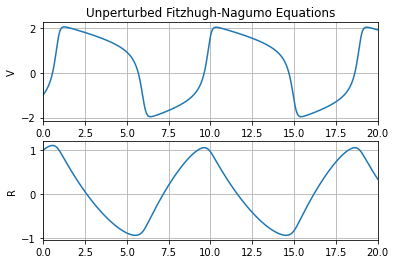
\includegraphics[width=0.7\textwidth]{fn-unperturbed.png}
  \caption{The Fitzhugh-Nagumo Equations with no perturbation.}
\end{figure}



\subsection{Lorenz 63}

The Lorenz-63 System is given as the following:

\begin{align*}
  \dot{x} &= \sigma (y - x)\\
  \dot{y} &= x ( \rho - z ) - y\\
  \dot{z} &= x y - \beta z
\end{align*}

For choices of parameters $\sigma=10,\, \rho=28,\, \beta=\frac{8}{3}$, this produces a chaotic attractor. Due to the chaotic behavior of the Lorenz attractor, even small changes in the right-hand side of its equations can cause significant change in the trajectory of the solution.

\begin{figure}[ht]
  \centering
  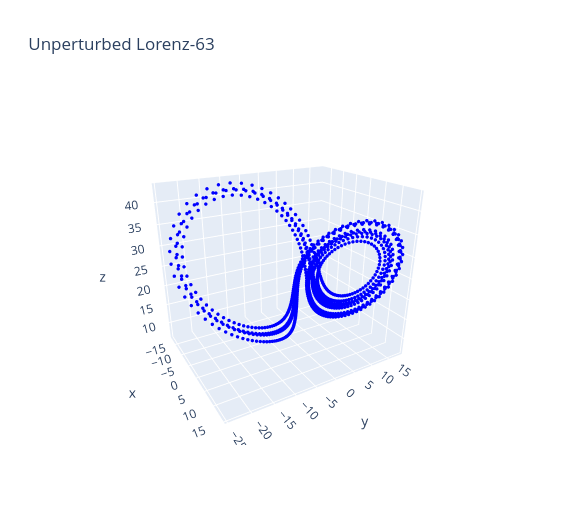
\includegraphics[width=0.9\textwidth]{lorenz-unperturbed.png}
  \caption{The Lorenz-63 System}
\end{figure}




\section{Results}

The methods described in \ref{methodology} are applied to perturbed versions of the two systems in \ref{examples} using the norms $L_1$, $L_2$, and $L_3$. The methods are then evaluated for convergence and runtime. As these methods are still a work in progress, evaluations will be based primarily upon qualitative behavior, rather than numerical evaluations of performance.


\subsection{Fitzhugh-Nagumo}

The Fitzhugh-Nagumo system exhibits oscillations for the chosen parameters and has stable behavior for small perturbations of its parameters.\cite{ramsay} However, perturbing the system with terms outside of the usual model is less well-understood. Thus, it will make a good test of how well the learning algorithm behaves in regions of parameter space where the function's behavior is not well known.

Taking $f_0$ to be the vector of right-hand side functions listed earlier, a basis of $[V^2, R^2]$ was chosen for the added terms so as to not overlap with terms already in the model. The ``true'' values were generated by numerically solving the system where $m^*(x)$ is defined as $m(x,\eta^*)$, and
$\eta = \big[\begin{smallmatrix}
  0.3 & 0\\
  0   & 0.05
  \end{smallmatrix}\big].$
Choosing $m^*$ to be of the same form as $m$ has some advantages, including that it allows for confirmation when the algorithm recovers the actual model used to generate the ground truth, as opposed to simply an $\eta$ that works. The algorithm is then set to train for $100$ iterations or until it converges.


\begin{figure}[ht]
  \centering
  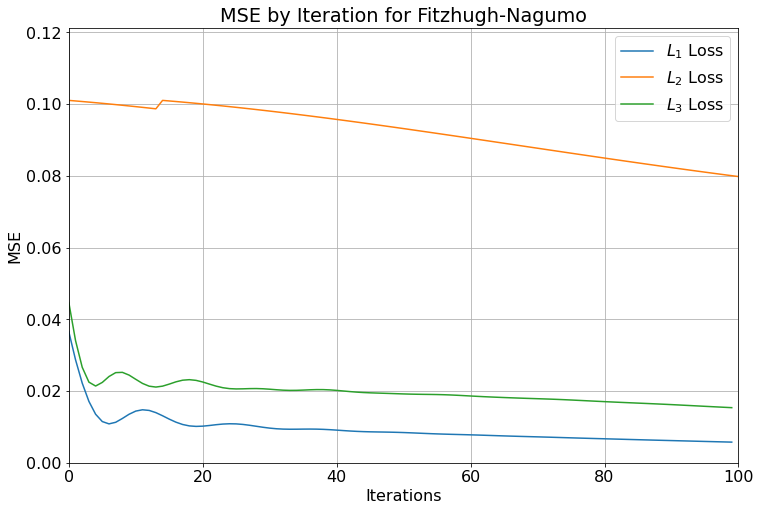
\includegraphics[width=0.9\textwidth]{mse-fn.png}
  \caption{Mean-Squared Error for learning the perturbed Fitzhugh-Nagumo model trained with different losses.}
\end{figure}

$100$ iterations is not long enough for any of these methods to converge, but it is enough to demonstrate that both $L_1$ and $L_3$ start decreasing the overall error and converging to the optimum rapidly. The $L_2$ loss behaves strangely and, looking forward to its long-term behavior, does not converge and eventually starts producing nonsense. This is likely due to errors in programming that will be fixed in the future. Nonetheless, the fact that the algorithm converges for this case is evidence that it is a powerful algorithm worth pursuing in future work.



\subsection{Lorenz 63}

The Lorenz-63 system is chosen to test the learning method presented primarily because of its chaotic dynamics. Though its chaotic attractor exists for a variety of parameter values, individual trajectories starting from the same initial point change drastically for slight changes in parameter values, making the task of guessing the effects due to small changes in parameters very difficult. Thus, if an algorithm learns perturbing terms reliably for the Lorenz system, it can be expected to do the same for most reasonable systems.

Taking $f_0$ to be the vector of the right-hand side functions listed earlier, a basis of $[y z, x^2]$ was chosen for the added terms so as to not overlap with terms already in the model. Similarly to before, $m^*(x)$ is defined as $m(x,\eta^*)$, and
$\eta = \big[\begin{smallmatrix}
  0 & 0.003\\
  0 & 0\\
  0.005 & 0
  \end{smallmatrix}\big].$

\begin{figure}[ht]
  \centering
  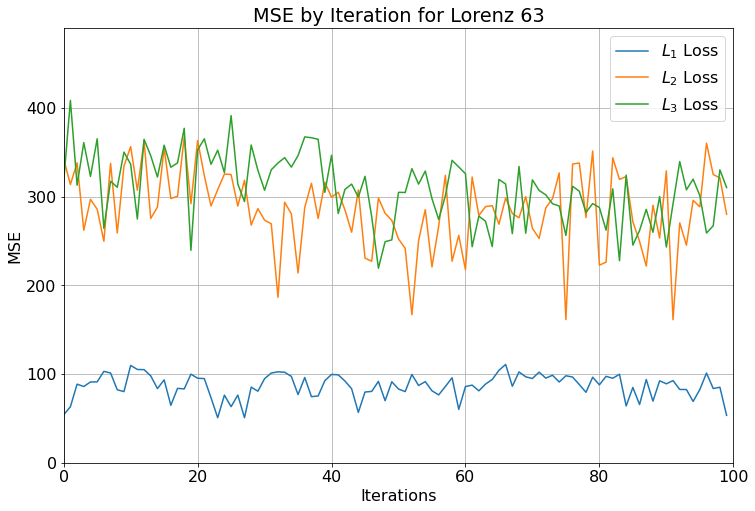
\includegraphics[width=0.9\textwidth]{mse-l63.png}
  \caption{Mean-Squared Error for learning the perturbed Lorenz 63 model trained with different losses.}
\end{figure}

The Lorenz system is in general much harder than other classical dynamical systems to apply numerical methods to, and these results are no exception. As mentioned previously, there is more work to be done in fully implementing the methods described in this paper, and the lack of convergence for any of these experiments is evidence that more methodological work may need to be done as well.



\subsection{Conclusions}

These results should be treated as preliminary and certainly not reflective of the full potential of the methods described in this report. There remains much tuning and reworking. For example, the $L_2$ loss appears to still have coding issues, as training with it with a better-tuned optimizer often causes it to converge to solutions that are neither optimal nor zero-gradient.

However, these results do show that the methods we have proposed have promise. Under certain conditions and given enough time, the algorithm often converges to the correct value of $\eta$. Moving forward with the easy-to-compute $L_2$ and expanding the algorithm to include larger bases could produce a very powerful algorithm for learning the parameters of Dynamical Systems.


\section{Additional Information}

The code used to obtain the results seen here can be found at \url{https://github.com/ariakoehler/dynamical-systems-learning}.





%% \pagebreak
\bibliographystyle{unsrt}
\bibliography{dynsys}


\end{document}
